\section{Resultados}
\label{sec:resultados}

\subsection{Planes comparados y alcance de los resultados}
El plan continuo de $60\,\mathrm{m^3/h}$ y la variante de $55\,\mathrm{m^3/h}$ comparten geometría, controles y escenarios. La comparación entre tasas utiliza la misma malla de $0{,}40\,\mathrm m$. La simulación adicional a $0{,}20\,\mathrm m$ comprueba la propuesta. Como la vertida única coincide con ella y la capacidad excluye una alternativa más rápida, hay dos cronogramas físicos distintos.

\subsection{Cronogramas de colocación y retiro de protecciones}
Ambos planes comienzan a las $10{:}00$ del $19$ de noviembre. En la Figura~\ref{fig:cronogramas-resultados}, la longitud de cada segmento representa el tiempo de colocación de una capa. La propuesta termina unas $10\,\mathrm h$ y $37\,\mathrm{min}$ después del inicio; la alternativa lenta, unas $11\,\mathrm h$ y $35\,\mathrm{min}$ después.
\begin{figure}[htbp]
  \centering
  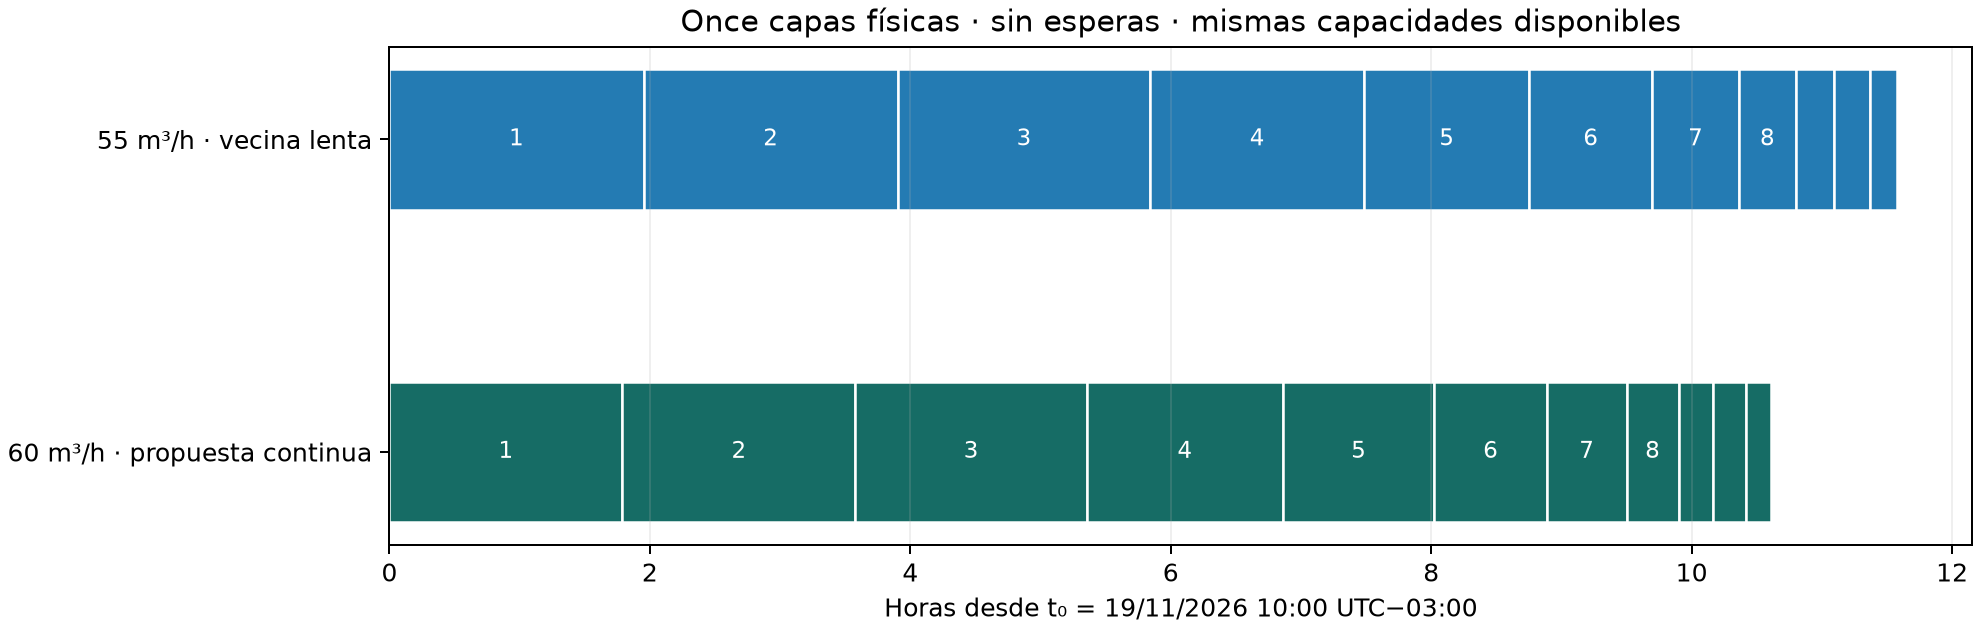
\includegraphics[width=0.98\linewidth]{Imagenes/resultados_02_CRONOGRAMAS.png}
  \caption{Secuencia continua de colocación de los dos planes finales}
  \label{fig:cronogramas-resultados}
  \captionsetup{skip=2pt}
  \caption*{Fuente: elaboración propia a partir del cronograma físico de las capas.}
\end{figure}
En el Anexo~\ref{an:detalles}, las Tablas~\ref{tab:cronograma-60} y~\ref{tab:cronograma-55} permiten trasladar la programación a cada frente. Los tiempos son horas desde $t_0$. Por ejemplo, en la propuesta el retiro de la última manta empieza a las $504\,\mathrm h$ en la primera capa y llega a la última a las $514{,}421\,\mathrm h$. Cada capa pasa entonces a sombra, que permanece hasta terminar el seguimiento.


\subsection{Probabilidades y máximos de cada plan}
La Tabla~\ref{tab:resultados-planes} reúne las duraciones, las probabilidades marginales y conjunta, y los extremos de cada conjunto de $24$ escenarios. Los dos planes cumplen a las $336$ y a las $672\,\mathrm h$. Entre ellos, la propuesta reduce la duración en $57{,}89\,\mathrm{min}$ sin aumentar la proporción de escenarios que exceden.
\begin{table}[htbp]
  \centering
  \caption{Duración, probabilidades y extremos del conjunto a $672\,\mathrm h$}
  \label{tab:resultados-planes}
  \small
  \setlength{\tabcolsep}{4pt}
  \begin{tabular}{lccccccc}
    \toprule
    Plan & $D$ [h] & $P_T$ & $P_\Delta$ & $P_f$ & Cumple & Mayor $M_T$ [$^\circ$C] & Mayor $M_\Delta$ [K] \\
    \midrule
    Propuesta base & $10{,}6129$ & $0$ & $0$ & $0$ & Sí & $47{,}4941$ & $16{,}5306$ \\
    Variante lenta & $11{,}5777$ & $0$ & $0$ & $0$ & Sí & $47{,}5128$ & $16{,}6011$ \\
    Propuesta fina & $10{,}6129$ & $0$ & $0$ & $0$ & Sí & $47{,}0322$ & $15{,}7202$ \\
    \bottomrule
  \end{tabular}
  \captionsetup{skip=2pt}
  \caption*{Fuente: elaboración propia a partir de las matrices finales de simulación.}
\end{table}
En la propuesta fina, la temperatura más alta fue de $47{,}03\,^\circ\mathrm C$ a las $126\,\mathrm h$, con \texttt{M4\_SS} y el clima de $2025$. El máximo diferencial, $15{,}72\,\mathrm K$, apareció a las $260{,}917\,\mathrm h$ con la misma curva y el clima de $2023$. En ese instante, el punto caliente alcanzó $40{,}73\,^\circ\mathrm C$ y el punto frío próximo al contorno, $25{,}01\,^\circ\mathrm C$.

La Tabla~\ref{tab:localizacion-maximos} identifica ambos puntos en coordenadas locales. Para el máximo absoluto de temperatura solo interviene $\vec x_T$; para el diferencial se necesitan $\vec x_T$ y $\vec x_{25}$ al mismo instante. La cota numérica de $4{,}40\,\mathrm m$ corresponde al contorno escalonado de la malla, mientras que el IFC alcanza $4{,}30\,\mathrm m$.
\begin{table}[htbp]
  \centering
  \caption{Escenarios, tiempos y posiciones de los extremos a $672\,\mathrm h$ ($M_T$ en $^\circ\mathrm C$ y $M_\Delta$ en $\mathrm K$)}
  \label{tab:localizacion-maximos}
  \small
  \setlength{\tabcolsep}{4pt}
  \begin{tabular}{L{1.5cm}L{1.2cm}L{1.15cm}L{1.2cm}L{1.8cm}L{3.3cm}L{3.3cm}}
    \toprule
    Plan & Métrica & Valor & Tiempo [h] & Escenario & $\vec x_T$ [m] & $\vec x_{25}$ [m] \\
    \midrule
    Propuesta base & $M_T$ & $47{,}4941$ & $125{,}000$ & \texttt{M4\_SS}, ERA5-$2025$ & $(2{,}000;0{,}000;4{,}400)$ & --- \\
    Propuesta base & $M_\Delta$ & $16{,}5306$ & $267{,}000$ & \texttt{M4\_SS}, ERA5-$2024$ & $(0{,}000;0{,}000;4{,}400)$ & $(-3{,}600;-8{,}800;0{,}025)$ \\
    Variante lenta & $M_T$ & $47{,}5128$ & $125{,}000$ & \texttt{M4\_SS}, ERA5-$2025$ & $(2{,}000;0{,}000;4{,}400)$ & --- \\
    Variante lenta & $M_\Delta$ & $16{,}6011$ & $267{,}000$ & \texttt{M4\_SS}, ERA5-$2024$ & $(0{,}000;0{,}000;4{,}400)$ & $(-3{,}600;-8{,}800;0{,}025)$ \\
    Propuesta fina & $M_T$ & $47{,}0322$ & $126{,}000$ & \texttt{M4\_SS}, ERA5-$2025$ & $(2{,}300;0{,}100;4{,}400)$ & --- \\
    Propuesta fina & $M_\Delta$ & $15{,}7202$ & $260{,}917$ & \texttt{M4\_SS}, ERA5-$2023$ & $(0{,}100;0{,}100;4{,}100)$ & $(3{,}700;-8{,}900;0{,}025)$ \\
    \bottomrule
  \end{tabular}
  \captionsetup{skip=2pt}
  \caption*{Fuente: elaboración propia a partir del cronograma y los resultados archivados de simulación.}
\end{table}


\subsection{Evolución del núcleo, del contorno y del diferencial}
La Figura~\ref{fig:curvas-resultados} sigue una sola realización, \texttt{M4\_SS} con el clima de $2024$, en las dos tasas y con idéntica resolución. El panel superior muestra el punto más caliente y el más frío de $S_{25}$; el central sigue una sonda fija del núcleo en $(0;0;2)\,\mathrm m$. El inferior muestra la diferencia simultánea y su límite.
\begin{figure}[htbp]
  \centering
  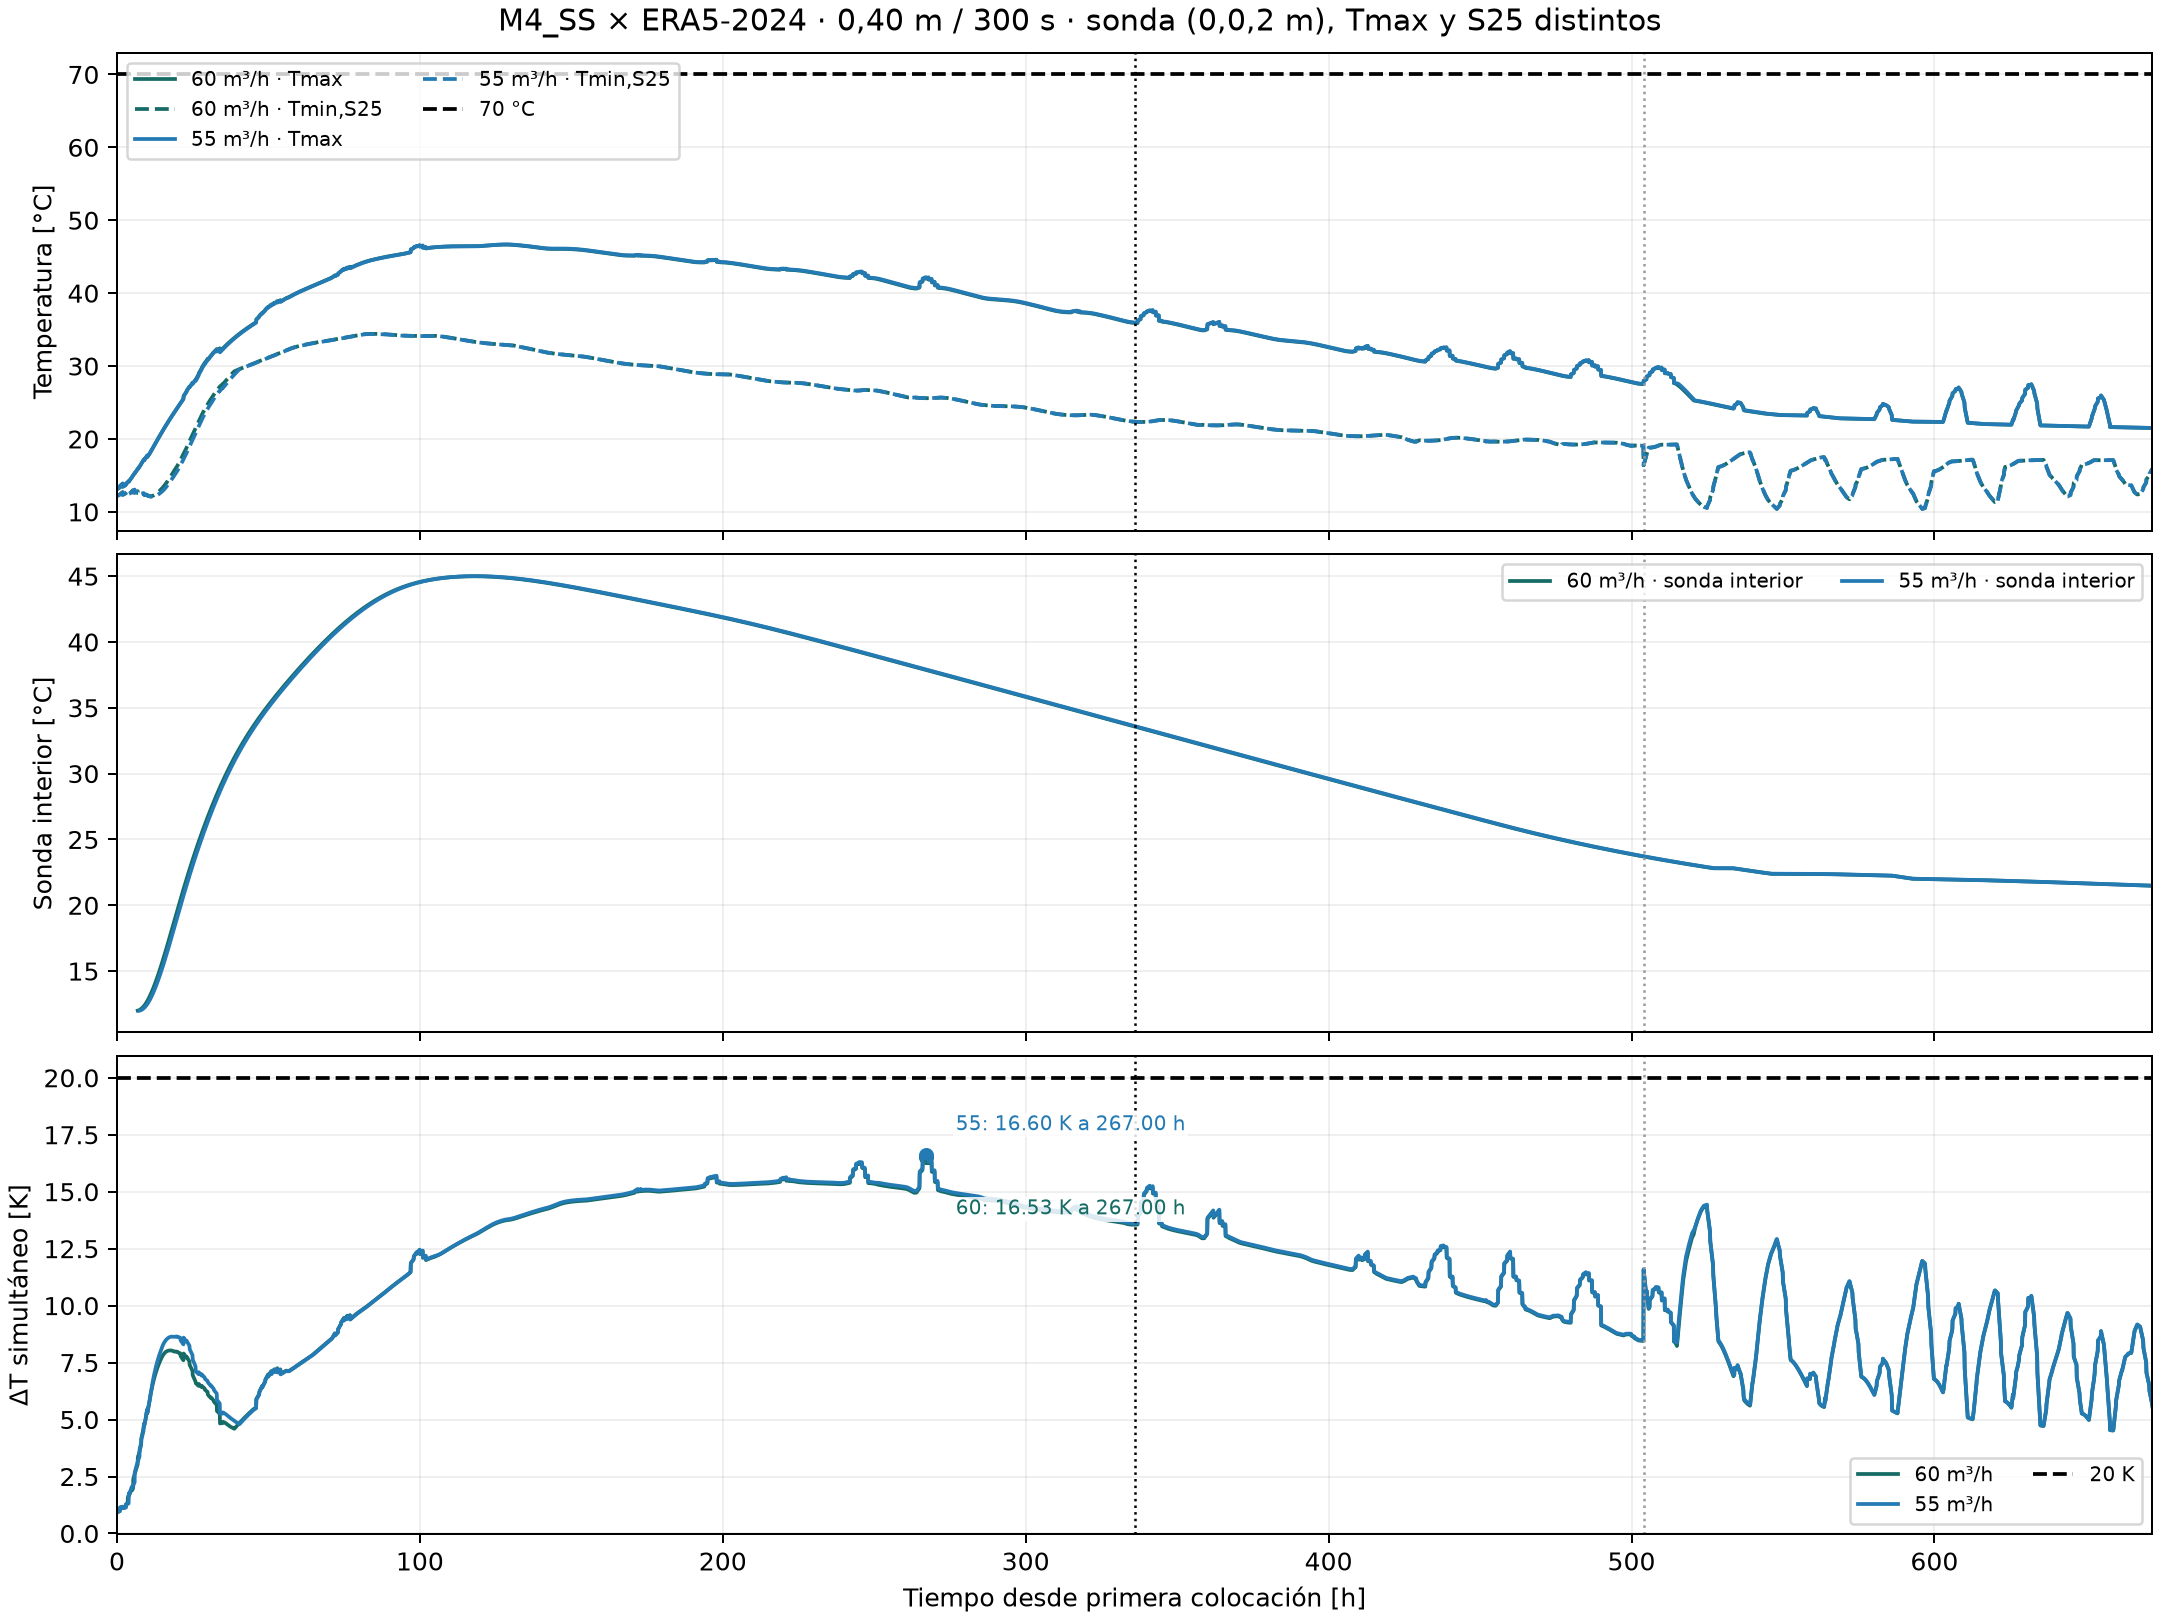
\includegraphics[width=0.98\linewidth]{Imagenes/resultados_03_CURVAS_COMPARABLES.png}
  \caption{Evolución térmica de una misma realización para los planes de $60$ y $55\,\mathrm{m^3/h}$}
  \label{fig:curvas-resultados}
  \captionsetup{skip=2pt}
  \caption*{Fuente: elaboración propia a partir de las historias térmicas de las simulaciones.}
\end{figure}
El núcleo se calienta durante las primeras edades y después se enfría más despacio que el contorno. A las $267\,\mathrm h$, el diferencial alcanza $16{,}53\,\mathrm K$ en la propuesta y $16{,}60\,\mathrm K$ en la alternativa lenta. Tras retirar la última manta crecen las oscilaciones cerca de la superficie. La línea de $504\,\mathrm h$ marca el primer retiro de esa manta.

\subsection{Campos térmicos y zonas críticas}
Los cortes de la Figura~\ref{fig:cortes-resultados} usan los mismos instantes y la misma escala de color. A las $267\,\mathrm h$ persiste una región cálida en la zona superior e interior, mientras que la base cede calor al suelo. A las $672\,\mathrm h$ el corte muestra un campo más uniforme. El punto frío que gobierna el diferencial en la malla base está cerca de $y=-8{,}80\,\mathrm m$, fuera del plano central; por eso se buscan los extremos en todo el volumen.
\begin{figure}[htbp]
  \centering
  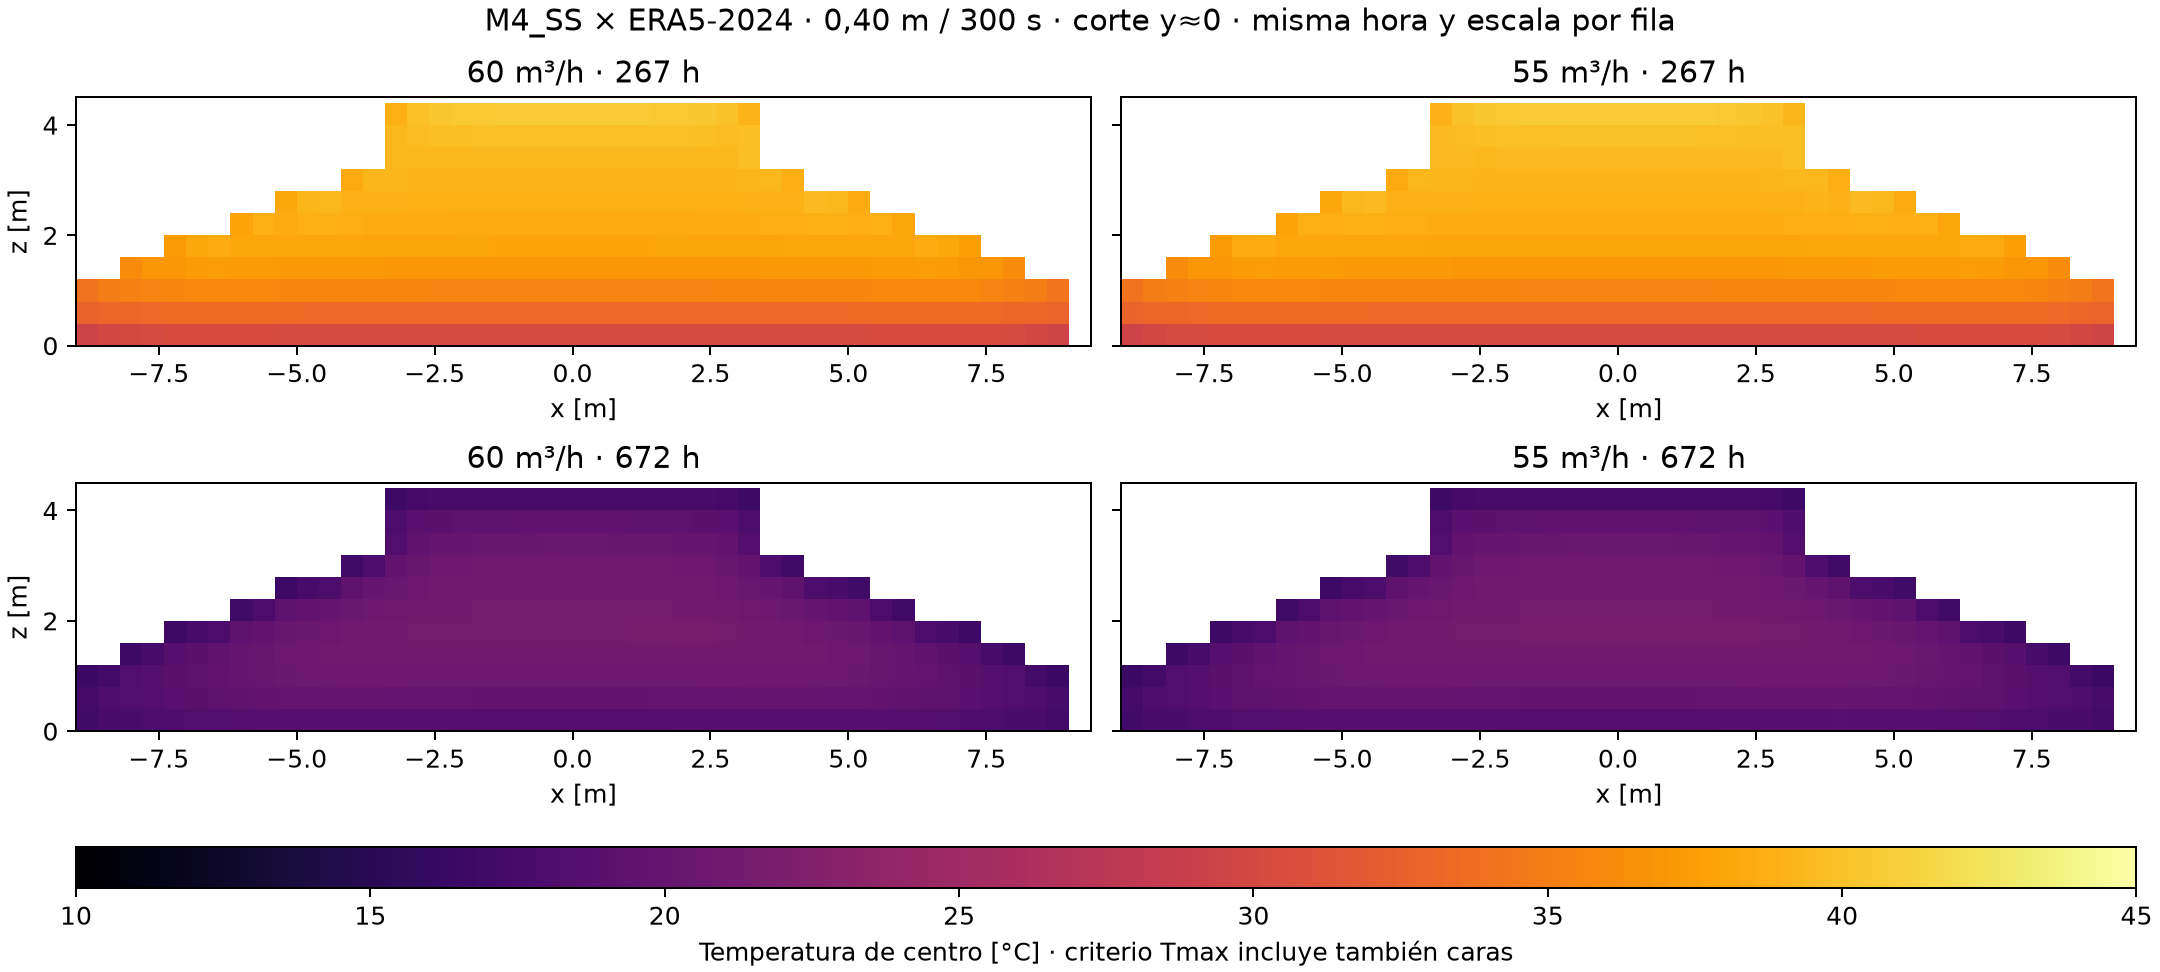
\includegraphics[width=0.98\linewidth]{Imagenes/resultados_04_CORTES_COMPARABLES_672H.png}
  \caption{Campos de temperatura en un corte central a $267$ y $672\,\mathrm h$}
  \label{fig:cortes-resultados}
  \captionsetup{skip=2pt}
  \caption*{Fuente: elaboración propia a partir de los campos de temperatura archivados.}
\end{figure}

\subsection{Relación entre duración, riesgo y desviaciones del plan}
En la Figura~\ref{fig:duracion-riesgo-resultados}, las dos tasas quedan por debajo de la línea del $5\,\text{\%}$ y la propuesta queda más a la izquierda por su menor duración. A tasa fija, el plazo es el mismo con las tres estrategias de protección, pero su resultado térmico cambia considerablemente.
\begin{figure}[htbp]
  \centering
  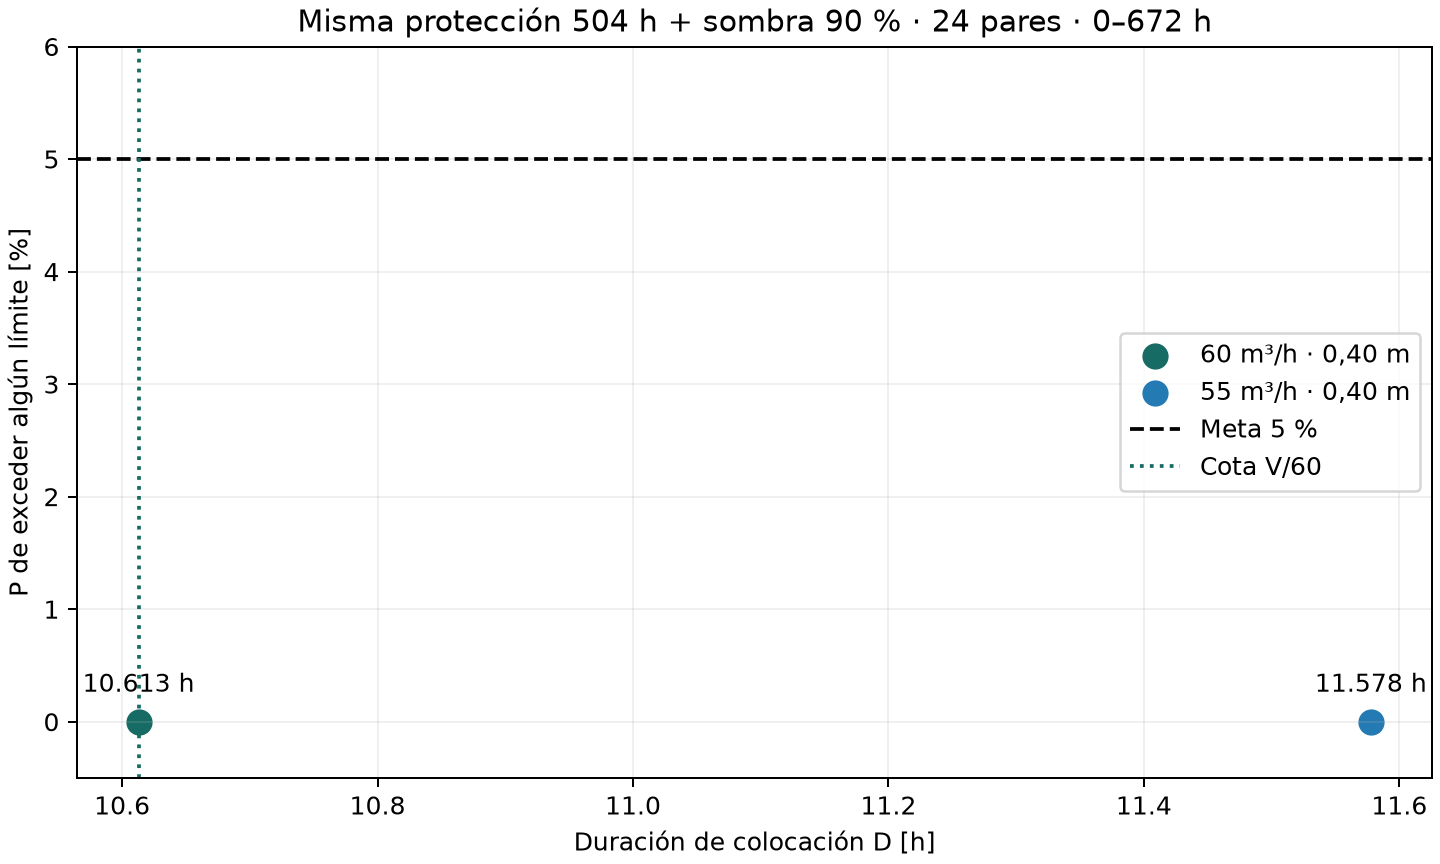
\includegraphics[width=0.90\linewidth]{Imagenes/resultados_01_D_VS_PROBABILIDAD.png}
  \caption{Duración y probabilidad conjunta de los planes finales, con la propuesta elegida en la cota $V/60$}
  \label{fig:duracion-riesgo-resultados}
  \captionsetup{skip=2pt}
  \caption*{Fuente: elaboración propia a partir de las duraciones y probabilidades de los planes.}
\end{figure}
Mantener la última manta hasta $504\,\mathrm h$ y prescindir de sombra produjo excedencias en los $24$ pares. Algunos máximos tardíos seguían pendientes, aunque la clasificación ya estaba decidida. Con sombra y retiro a $360\,\mathrm h$ excedieron $5$ de los $24$ pares ($20{,}83\,\text{\%}$). Al combinar la sombra con el retiro a $504\,\mathrm h$, ninguno excedió. Las cifras corresponden a la misma malla base, el mismo horizonte de $672\,\mathrm h$ y una duración de colocación de $10{,}6129\,\mathrm h$.

\subsection{Sensibilidades y fundamento de la elección}
La Figura~\ref{fig:sensibilidad-resultados} compara el máximo diferencial de cada escenario entre las dos mallas. El mayor cambio observado, $0{,}882\,\mathrm K$, deja la elección del mismo lado del umbral en los $24$ pares. La sensibilidad a los pesos de la Tabla~\ref{tab:sensibilidad-pesos} conserva también la decisión.
\begin{figure}[htbp]
  \centering
  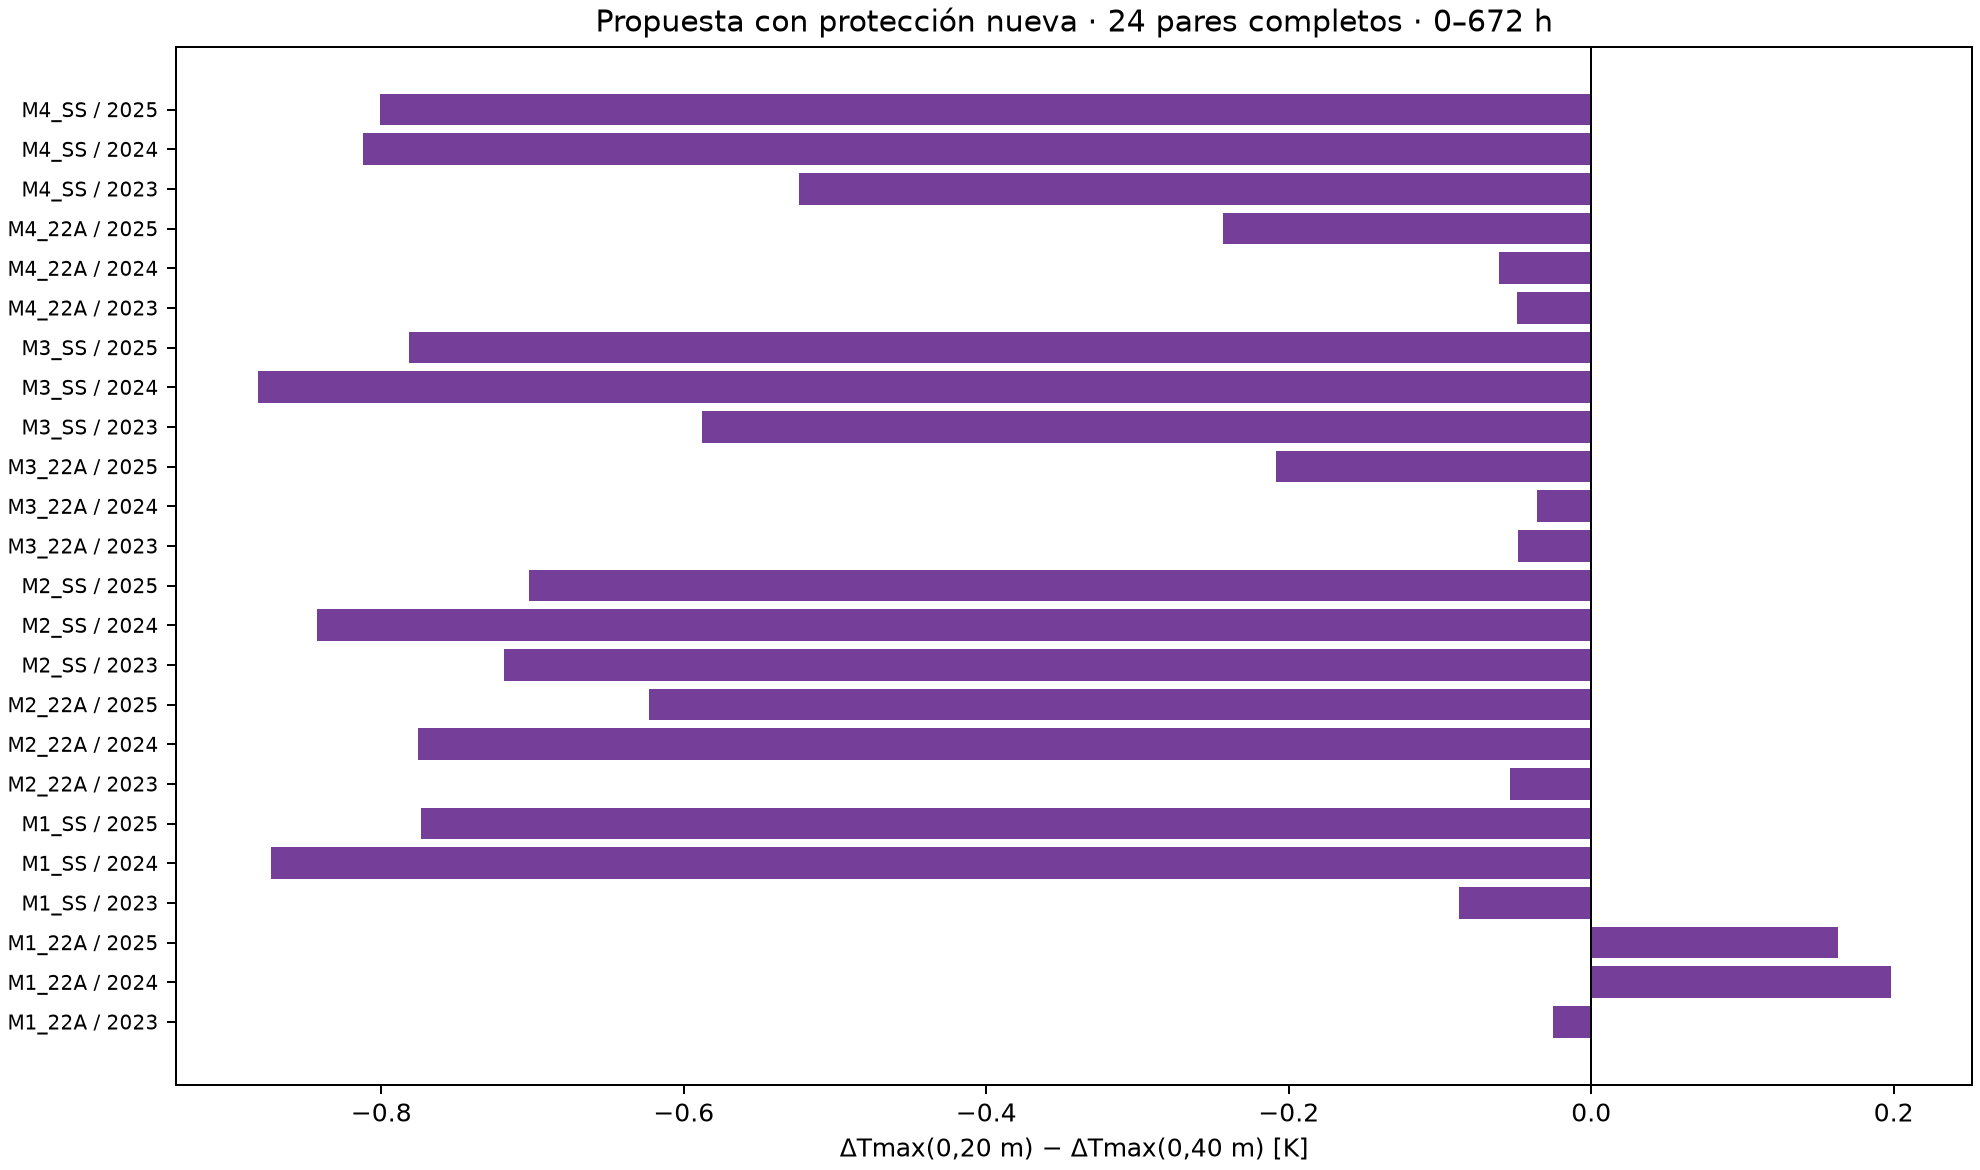
\includegraphics[width=0.95\linewidth]{Imagenes/resultados_05_SENSIBILIDAD_24_PARES.png}
  \caption{Cambio del diferencial máximo entre mallas para los $24$ escenarios de la propuesta}
  \label{fig:sensibilidad-resultados}
  \captionsetup{skip=2pt}
  \caption*{Fuente: elaboración propia a partir de las comparaciones de cada escenario en ambas mallas.}
\end{figure}
Cada barra compara máximos de una misma realización. Promediar primero los campos de temperatura suavizaría las diferencias entre años y curvas y podría ocultar precisamente una excedencia. La elección utiliza la duración física y la distribución de máximos individuales.
